\documentclass[12pt]{article}
\usepackage{geometry} % see geometry.pdf on how to lay out the page. There's lots.
\geometry{a4paper} % or letter or a5paper or ... etc
\usepackage{graphicx}
\usepackage{cite}
\usepackage{color}
\usepackage{bm}
\usepackage{amsmath}
\usepackage[fleqn,tbtags]{mathtools}
\usepackage{amsfonts}
\usepackage{ulem}
\usepackage{hyperref}
\usepackage{float}
\usepackage{textcomp}

\newcommand{\Matrix}[1]{\ensuremath{\mathtt{#1}}}

% \geometry{landscape} % rotated page geometry

\title{Response to the reviewers of the manuscript ``Explicit meshfree $u-p_w$ solution of the dynamic Biot formulation at large strain"}
\author{Pedro Navas, Miguel Molinos, Miguel M. Stickle, \\ Diego Manzanal, Angel Yag\"ue and Manuel Pastor}


%\date{} % delete this line to display the current date

%%% BEGIN DOCUMENT
\begin{document}

\maketitle
%\tableofcontents

We  are grateful to the reviewers for taking their time  to review our work. Their comments have helped us to improve the paper. Changes to the original manuscript are given in  color \textcolor{red}{red} for corrections and  \textcolor{blue}{blue} for modified text in the revised version.  A detailed response to both reviewers is given below.

\section*{Response to Reviewer \#1}
{\it
This manuscript presents a meshfree formulation for dynamic poromechanics at large strains. The formulation is based on a reduced two-field ($u-p_w$) form in which the relative acceleration between the solid and fluid phases are neglected, which may be justified for low-frequency loading. For temporal discretization of the formulation, the authors use an explicit Newmark method, and for spatial discretization, they use a local maximum entropy (max-ent) in the Optimal Transportation Framework (OTM). The resultant formulation is studied with two types of numerical examples: consolidation and vertical cut. The methodology studied in this paper is certainly attractive. I'm not sure, however, whether the numerical method and formulation indeed have novelty that deserves publication. For example, the explicit time integration scheme in this work, which the authors phrased as "novel," appears to be just a standard explicit Newmark scheme. Other aspects were also adopted from existing works. For example, the two-field formulation for low-frequency dynamics was first proposed by Zienkiewicz and co-workers, and the local max-ent OTM for poromechanics was proposed by the authors a few years ago. So to be quite honest, I don't really find anything new in terms of the numerical method and formulation.}\\

We would like to thank the reviewer to take his/her time to assess our manuscript. We agree that Max-Ent OTM methodology within poromechanics problems and the traditional predictor-corrector Newmark scheme are not new developments. However, the novelty lies on the application of this dynamic $u-p_w$ formulation with this explicit scheme at finite strains. The most recent works on explicit poromechanics schemes are written in a Forward-Euler manner (\cite{ZHANG_et_al_2009}), that shows less stability than the predictor-corrector schemes. This two-step methodology allows to reach time steps closer than the CFL condition with accurate results. Moreover, contrary to other similar works, the methodology proposed in this manuscript is written in a finite strain approach, not seen in the most recent works of dynamic poromechanics (unless the ones the reviewer cites of the same authors).\\

\textit{Instead, I found that the results of the numerical examples are interesting and may yield new findings if they are analyzed more deeply. Examples of potential discussion topics include:}:

\begin{enumerate}

\item \textit{Is the CFL condition given in Eq. (29) valid for the current approach? The authors didn't show evidence whether Eq. (29) works accurately for the current method. The answer to this question is not so obvious for the current meshfree method.}\\

The discretization size, $h$, is an interesting topic when dealing with explicit schemes in the OTM methodology. Although the neighborhood or influence radius is larger than in the traditional FEM~\cite{li2010}, we should take $h$ as the distance between the current node and the closest one since it is the more limiting one. Indeed, the employment of $h$ in this manner has been treated in different OTM researches as well as in the ``Vertical Cut" example as suggested by the reviewer later. This explanation has been included in the revised version of the original manuscript.


\item \textit{For the numerical examples considered, is the explicit method really more efficient than an implicit method with larger time steps? Actually explicit methods are much easier to use as the authors explained, but their maximum time step size allowed is often too small for practical purposes. This is why many researchers have studied semi-implicit and fully-implicit methods mentioned in the Introduction. In my opinion, the authors did not fully discuss the drawbacks of the explicit method. I would recommend that the authors show how the explicit method become unstable as the time step becomes larger (also related to my question 1).}\\

We agree with the reviewer's opinion on this explanation: the explicit schemes are robust and feasible for fast phenomena while larger simulations require excessive steps due to the limitation of the time step. Following the reviewer's recommendation, an assessment of the time step limitation has been carried out.


\item \textit{Fig. 2 -- this quasi-static monotonic loading consolidation problem may be regarded as a problem with low-frequency loading. They why do the three formulations show such significant differences?}\\

The studied problem cannot be considered as a low-frequency one since the load is applied quickly: a pressure is applied incrementally from 0 to 2-8 MPa from the beginning until $t_f=$0.05 seconds, when the pressure is kept constant. This load was previously employed by Navas \textit{et al.}~\cite{Navas:17b,Navas:17c}, adapting the one proposed by Li, Borja and Regueiro~\cite{LiBorja2004} when inertial terms are involved.

If we assume that the ramped part of the load can be approximated by a quarter of sinusoidal load, the associated period $T$ would be four times $t_f$, \textit{i.e.}, 0.2 seconds. Taking into account that $\omega=2\pi/T$, we can consider a frequency, $\omega$, of 31.5 rad/s, which can be regarded as a medium-high frequency loading. This relatively fast loading process explains the discrepancies appearing in Fig 2.

\item \textit{Fig. 5 -- the authors studied the (in)applicability of this figure using numerical examples, and this was the most interesting point to me. But it is not explained how the zone boundaries were originally derived by Zienkiewicz and co-workers, and please elaborate on how they were derived. I also suggest that the authors connect this to explain the results in Fig. 2. }\\

Zienkiewicz and coworkers examined in 1980 the range of validity of the different formulations to represent the behavior of saturated porous media, i.e. $u-w, u-p_w \text{ (dynamic)}, u-p_w \text{ (consolidation)}$,  under dynamic or quasi-static loads by means of an analytical study of a soil layer subjected to a periodic surface loading. 

The principal result obtained by Zienkiewicz and coworkers in 1980 is Fig. 5 of the present work. This figure was derived as follows: 

\begin{enumerate}
    \item For a fixed set of elastic parameters of the soil layer, densities, compressibility and porosity, the different formulations were evaluated for a large range of permeability and load frequency.
    \item In Zone I the three formulations give the same results, up to a discrepancy of $3\%$. This zone can be considered for slow phenomena.
    \item In Zone II the $u-w, u-p_w \text{ (dynamic)}$ formulations agree, up to a discrepancy of $3\%$, but $u-p_w \text{ (consolidation)}$ display different result.
    \item In Zone III the three formulations display different results. This zone can be considered for extremely rapid phenomena. 
\end{enumerate}

As suggested by the reviewer, results in Fig. 2 have been linked with Fig 5. of the manuscript. By considering the set of parameters displayed in Table 1, the large deformation consolidation validation case falls within Zone III. As we mentioned before, we can approximate the frequency of the load to 31.5 rad/s, which is a considerable high frequency, taking into account the nature of the problem. From the problem parameters, it can be obtained $\pi_1 \approx 1.0$ and $\pi_2 \approx 1.0e3$, what is plotted in the following figure:

\begin{figure}[h]
\centering
  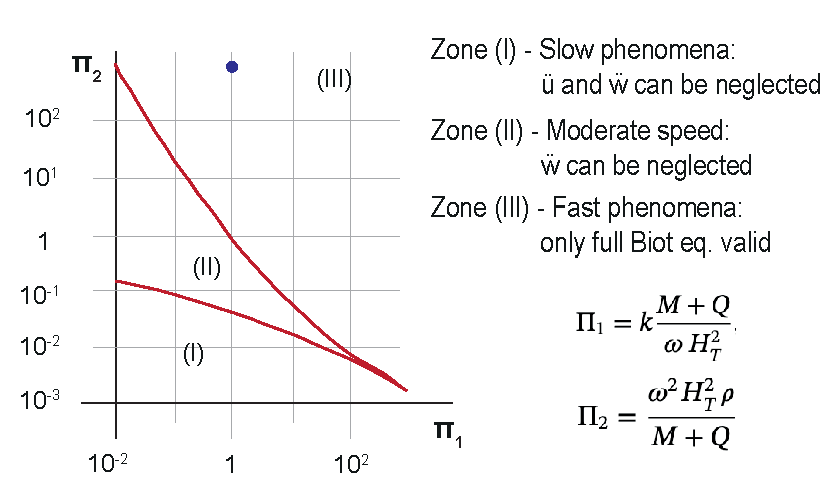
\includegraphics[width=0.75\textwidth]{Reviews/zienk_2.pdf}
\caption{Location of Large Deformation Consolidation problem in the Zienkiewicz's graph.}
%\label{fig:1}       % Give a unique label
\end{figure}



\item \textit{For the ``Vertical Cut" example, I suggest the authors use two different spatial discretization sizes (i.e. different "h"s) and numerical show whether the problem is mesh-sensitive and how the maximum time step size changes according to the value of "h" (and whether Eq. (29) holds accurately).}\\

Further analysis of this example has been added to the original section within the manuscript.\\

\end{enumerate}
 
\textit{Other typos, etc.}

\begin{enumerate}
    \item \textit{"The additional novelty" in abstract: again, it's unsure whether the numerical method in this paper is really novel.}\\
    
    As we mentioned before, the novelty is not the employment of an explicit scheme but the development of a predictor-corrector scheme at large strain. This has been modified in the abstract of the manuscript.
    
    \item \textit{Researches (throughout the manuscript) $\rightarrow$ research (it's an uncountable noun)}\\.

    Fixed.

    \item \textit{validation (throughout the manuscript) $\rightarrow$ verification (it'd be more appropriate to use "verification" for what the authors carried out, according to their definitions in computational engineering explained by Babuska and Oden CMAME 2004).}\\

    Fixed.

    \item \textit{$K_T$ in Eq. (8) is not consistent with the definitions in the nomenclature.}\\
    
    Fixed.
    
    \item \textit{Of coarse $\rightarrow$ of course (p. 10)}\\
    
    Fixed.
    
    \item \textit{Final paragraph: Galerking $\rightarrow$ Galerkin.}\\

    Fixed.
    
    \item \textit{Citation errors [16,?,?].}\\
    
    Fixed.
    
    \item \textit{It'd be better to make the units in Fig. 9 consistent with those in other examples.}\\
    
    Fixed.
    
\end{enumerate}


\section*{Response to Reviewer \#3}

\textit{The manuscript JCPM-D-21-00035 develops an explicit meshfree u-p formulation for liquid water saturated porous media at large strain in dynamics. The model is then used to simulate consolidation of a soil column and a square domain loaded on the top by a rigid footing. This manuscript follows other papers published in particular by the first and the senior authors, is well written, original and merits publication almost as it is.}\\

The reviewer\textquotesingle s positive commentaries are greatly appreciated.\\

\textit{The following minor remarks are shared with the authors. :}\\

 \begin{enumerate}
\item \textit{Section 2: eqs.2 and 5 are written for water saturated materials, while eqs.1,3,6,7,10 and eq. at line 54 page 3 are for variably saturated materials. The authors are invited to choose the formulation to be used and to be consistent with that.}\\

We agree with the reviewer. Eqs. 2 and 5 have been moved after the definition of saturated media (After Eq. 6)

\item \textit{Eq.8 could be moved after eq.2, because $\alpha$ appears in eq.2.}\\

Since this chapter has been rephrased, the definition of $\alpha$ is made immediately after its appearance.

\item \textit{Line 32, page 3, right column: ''more rigid'' could be substituted with ''less deformable'' (or the sentence could be rephrased taking into account that the solid grains are considered incompressible with respect to the solid skeleton).}\\

Fixed

\item \textit{Line 39 , page 3, right column: krw is not used in the equations above and can be deleted.}\\

Fixed

\item \textit{Line 18, page 6, right column: check if the citation of [15] is correct.}\\

This citation has been revised. Indeed, this work of Sanavia and coworkers does not deal with large strain.

\item \textit{Rephrase the sentence at lines 36-38 page 8 left column (''Because of this fac… 0.3 seconds''.}\\

It has been rephrased as follows:
``In addition, the existence of displacements larger than the final settlement between 0.18 s. and 0.3 s. can be attributed to the above observation regarding the u-w formulation."

\item \textit{Clarify ''stabilized and unstabilized'' at line 34 page 8 right column.}\\

These terms do not correspond with this figure. They were deleted.

\item \textit{Fig.10, water pressure for the dilatant material: add a comment because negative pressures are shown (which invokes a variably saturated porous media model).}\\

This paragraph has been added in order to expose the academic purpose of this example, being necessary the unsaturated one in order to capture the negative pore pressure behavior:

``In the case of $\psi=20^\circ$, it can be noted in Fig. 11 that the negative water pressure within the shear band is smaller than zero, indicating the possible occurrence of cavitation when lower values of -98986 Pa (at ambient temperature) are reached. This phenomenon should be modeled by extending the formulation of this paper to unsaturated conditions in order to properly capture this phenomenon".

\item \textit{Nomenclature: $\beta$ and $\gamma$ are time integration parameters and LME parameters. The meaning is clear, but, for sake of clarity, different symbols could be adopted. If the author agrees with this remark, some equations need to be modified accordingly.}\\

Changed to $\beta__{LME}$ and $\gamma__{LME}$.

\item \textit{Typos: ''hidromechanical'' (page 1, line 27, second column). ''Figs.'' (line 15 page 10 right column). The citation at line 54 page 12.}\\

Fixed

\end{enumerate}


\bibliographystyle{unsrt}
\begin{thebibliography}{10}

\bibitem{ZHANG_et_al_2009}
Zhang, H.W. and Wang, K.P.  and Chen, Z.
\newblock{Material point method for dynamic analysis of saturated porous media under external contact/impact of solid bodies}.
\newblock{Computer Methods in Applied Mechanics and Engineering}, 2009.

\bibitem{Navas:17b}
Navas, P., Sanavia, L., L{\'{o}}pez-Querol, S., Yu, R.C.: {Explicit meshfree
  solution for large deformation dynamic problems in saturated porous media.}
\newblock Acta geotechnica \textbf{13}, 227--242 (2018).
\newblock \doi{10.1007/s11440-017-0612-7}.

\bibitem{Navas:17c}
Navas, P., Sanavia, L., L{\'{o}}pez-Querol, S., Yu, R.C.: u-w formulation for
  dynamic problems in large deformation regime solved through an implicit
  meshfree scheme.
\newblock Computational mechanics \textbf{62}, 745--760 (2018).
\newblock \doi{10.1007/s00466-017-1524-y}.

\bibitem{LiBorja2004}
Li, C., Borja, R.I., Regueiro, R.A.: {Dynamics of porous media at finite
  strain}.
\newblock Computer Methods in Applied Mechanics and Engineering
  \textbf{193}(36-38), 3837--3870 (2004).
\newblock \doi{10.1016/j.cma.2004.02.014}

\bibitem{li2010}
Li, B., Habbal, F., Ortiz, M.: {Optimal transportation meshfree approximation
  schemes for fluid and plastic flows}.
\newblock International Journal for Numerical Methods in Engineering
  \textbf{83}(June), 1541--1579 (2010).
\newblock \doi{10.1002/nme}



\end{thebibliography}

\end{document}
  